% Emphasize we only handle even m case.

%In 3D we can make use of the decoupling of our
%2D arrays to reduce memory usage to 1/4 of the explicit usage in the
%standard case and 4/9 in the centered case.

\documentclass[final]{siamltex}
\usepackage[lined,algonl,boxed]{algorithm2e}

\usepackage{hyperref}
\usepackage{mathdef}

\let\orightarrow\rightarrow
\let\omapsto\mapsto
\usepackage{breqn}
\let\rightarrow\orightarrow
\def\longrightarrow{\relbar\joinrel\joinrel\joinrel\orightarrow}
\let\mapsto\omapsto
\usepackage{hyperbreqn}

\def\be{\begin{dmath*}}
\def\ee{\end{dmath*}}
\def\bel{\begin{dmath}}
\def\eel{\end{dmath}}
\def\bec{\begin{dmath*}[compact]}
\let\eec\ee
\def\belc{\begin{equation}}
\def\eelc{\end{equation}}

\def\bg{\begin{dgroup*}}
\def\eg{\end{dgroup*}}
\def\bgl{\begin{dgroup}}
\def\egl{\end{dgroup}}
\def\bs{\begin{dsuspend}}
\def\es{\end{dsuspend}}
\def\no{\hiderel}

\def\Re{\mathop{\rm Re}\nolimits}
\def\Im{\mathop{\rm Im}\nolimits}

\begin{document}

%\title{Implicit Dealiasing of Fourier-Based Convolutions}
\title{Efficient Dealiased Convolutions without the Padding}
\author{John C. Bowman and Malcolm Roberts}
\maketitle

\begin{abstract}
An algorithm is described for calculating dealiased linear convolution sums
without the expense of conventional zero-padding or phase-shift
techniques. For one-dimensional in-place convolutions, the memory
requirements are identical with the zero-padding technique, with the important
distinction that the additional work memory need not be contiguous with the
data. This decoupling of the data and work arrays significantly reduces
the memory and computation time required to evaluate higher-dimensional
in-place convolutions. The technique also allows one to efficiently dealias the
hyperconvolutions that arise on Fourier transforming cubic and higher powers.
Implicitly dealiased convolutions can be built on top of state-of-the-art
fast Fourier transform libraries: vectorized multidimensional implementations
for the complex and centered Hermitian (pseudospectral) cases have
been implemented in the open-source software {\tt fftw++}.
\end{abstract} 

\begin{keywords} 
dealiasing, zero padding, convolution, hyperconvolution, fast Fourier transform,
pseudospectral method, in-place transform, bit reversal
\end{keywords}

\begin{AMS}
65R99,65T50
%15A15, 15A09, 15A23
\end{AMS}

\pagestyle{myheadings}

%use out-of-place Fourier transforms where possible (percent?)

% decoupling is more convenient for the user, 
% 

%padding to smooth data vs. chirp-z algorithm

%highly optimized

%avoids inconvenience of and extra copying required by zero padding

% CRAY power-of-2 stride issue
% Supports efficient convolutions of power of 2 sizes
%

% Think about parallelization issues (another advantage of removing zeros).

\bibliographystyle{siam}

\section{Introduction}
Discrete linear convolution sums based on the fast Fourier transform
(FFT) algorithm \cite{Gauss1866,Cooley65} have become important tools
for image filtering, digital signal processing, and correlation
analysis. They are also widely used in computational physics to solve
nonlinear partial differential equations, such as the Navier--Stokes
equations, in periodic domains. In some of these applications, notably
direct numerical pseudospectral simulations of fluid turbulence,
memory usage is a critical limiting factor, and in-place
multidimensional Fourier transforms are used to reduce the memory
footprint of the required spectral convolutions.

Because the discrete convolution, which produces cyclic output from cyclic
input, is applied to nonperiodic (wavenumber-space) data, it is important
to remove aliases from the convolution. Typically the data array is
extended by padding it with enough zeros so that the wave beats of the
the positive frequencies cannot wrap around and contaminate
the negative frequencies. A cyclic convolution $\sum_{p=0}^{N-1} f_p g_{k-p}$ is then performed using a
correspondingly larger Fourier transform size $N$. If the cost of 
computing a complex Fourier transform of size $N$ is asymptotic to 
$K N\log_2 N$ as \hbox{$N\goesto\infty$} (the lowest bound currently 
achievable is $K=34/9$ \cite{Johnson07,Lundy07}), the asymptotic cost of
computing the convolution of two vectors of unpadded length $m$ is
$6Km\log_2 m$ (using $N=2m$ and three Fourier transforms).
Another important case in practice is the centered Hermitian~1D convolution,
$\sum_{p=-m+1}^{m-1} f_p g_{k-p}$, which requires $\fr{9}{2}Km\log_2 m$
operations.
Alternatively, phase shift dealiasing \cite{Patterson71,Canuto} can be used
to cancel out the aliasing errors between two convolutions with two
different phase shifts. However, this second technique is rarely used in
practice, since in addition to doubling the memory requirements, it is
computationally more expensive, requiring for a centered Hermitian convolution
$6K m\log_2 m$ operations.

An explicit application of the zero-padding technique involves the rather
obvious inefficiency of summing over a large number of data values that
are known {\it a priori\/} to be zero.
However, it is first worth understanding the following answer 
provided by Steven G. Johnson to a frequently asked question in the
community about avoiding this unnecessary
expense \cite{http://www.fftw.org/pruned.html}:
\begin{quotation}\label{quote}
{\it
The most common case where people seem to want a pruned FFT is for
zero-padded convolutions, where roughly 50\% of your inputs are zero (to
get a linear convolution from an FFT-based cyclic convolution). Here, a
pruned FFT is hardly worth thinking about, at least in one dimension. In
higher dimensions, matters change (e.g. for a 3d zero-padded array about
1/8 of your inputs are non-zero, and one can fairly easily save a factor of
two or so simply by skipping 1d sub-transforms that are zero).
}
\end{quotation}

The reasoning behind the assertion that such one-dimensional pruned FFTs
are not worth thinking about is that if $m$ of the $N$ inputs are nonzero,
the computational cost is reduced only from $N\log N$ to $N\log m$.
For example, if $m=N/2$, the savings is a minuscule $1/\log_2 N$.
Nevertheless, in this work we demonstrate that pruning the zero-padded
elements of one-dimensional convolutions is indeed worth thinking about,
primarily because it provides a more effective building block for constructing
multidimensional convolutions.

The key observation is that, although the memory usage of our implicitly
padded 1D convolution is identical to that for a conventional explicitly
padded convolution, the additional temporary memory need not be contiguous
with the user data.  In a multidimensional context, this external work
buffer can be reused for other one-dimensional convolutions.
As a result, for dimensions greater than one,
an implicitly dealised standard convolution $\sum_{p=0}^{m-1} f_p g_{k-p}$
asymptotically uses half of the
memory required by explicit padding. For the case where the Fourier origin is
centered in the domain, memory usage is reduced by one third.
Of course, if memory savings alone were the goal, these savings could
also be achieved with explicit zero padding by copying the data for the
innermost convolution to an external padded buffer, but such extra data
communication degrades performance. The fact that our
one-dimensional convolution does not require this extra copying is the key
feature that was exploited to obtain simultaneous improvements in memory
usage and speed.

Nevertheless, the task of writing an efficient implicitly dealiased
one-dimensional convolution is onerous, particularly if one tries to
%platform-adaptive
compete with an explicitly problem-dependent and architecture-adaptive
FFTW algorithm such as the award-winning \cite{FFTW} library, which
empirically predetermines a near optimal butterfly graph
%FIXME:REForDEFN
%Standard term from graph theory/FFT literature 
%(e.g. see butterfly diagram in Wikipedia). Maybe add
%Alan V. Oppenheim, Ronald W. Schafer, and John R. Buck, Discrete-Time Signal Processing, 2nd edition (Upper Saddle River, NJ: Prentice Hall, 1989)
at each subdivision. Effectively one wants to perform
the first FFT subdivision manually, dropping the zero terms and
leaving the inner transforms to be computed with the usual library
routine. But this places an artificial restriction, at least at the
highest subdivision, on the possible adaptive algorithm that can be
used. Fortunately, there are a number of features of our algorithm
that help to offset this disadvantage. First, if the goal is to
produce a convolution, bit-reversal for the manual (highest)
subdivision is unnecessary: the scrambled Fourier subtransforms of the
two input vectors can be multiplied together as they are produced
(perhaps while still accessible in the cache). Second, the implicit
method allows most of the subtransforms for an in-place convolution to
be computed as out-of-place transforms, which execute faster than
in-place transforms since they require no extra (pre-, post-, or
interlaced) bit-reversal stage.  These savings helped keep our
one-dimensional in-place implicit convolution competitive with the
explicitly padded convolution based on the same highly optimized
library.

%Add outline
Implicit padding can be used to efficiently dealias hyperconvolutions
such as $\sum_{p=0}^{m-1}\sum_{q=0}^{k-p} f_p g_q h_{k-p-q}$. 
For example, in section~\ref{hconv} we compute a centered Hermitian
biconvolution.

\section{Implicitly dealiased 1D convolutions}
\subsection{Complex convolution}
The Fourier origin for standard convolutions is located at index zero.
Therefore, input data vectors of length $m$ must be padded with zeros to
length $N\ge 2m-1$ to prevent mode $m-1$ from beating with itself to
contaminate mode~$N=0\mod N$. However, since FFT sizes with small prime
factors in practice yield the most efficient implementations, it is normally
desirable to extend the padding to $N=2m$.

In terms of the $N$th primitive root of unity, $\zeta_N\doteq \exp\(2 \pi
i/N\)$, (here $\doteq$ indicates a definition), the unnormalized backwards
discrete Fourier transform of a complex vector
$\{U_k: k=0,\ldots,N\}$ may be written
$$
u_j\doteq\sum_{k=0}^{N-1}\zeta_N^{jk} U_k\qquad j=0,\ldots,N-1.
$$
The fast Fourier transform method exploits the properties that
$\zeta_N^r=\zeta_{N/r}$ and $\zeta_N^N=1$.

If $U_k=0$ for $k \ge m$, one can easily avoid looping over the
unwanted zero Fourier modes by decimating in wavenumber:
\belc
u_{2\ell}
=\ds\sum_{k=0}^{m-1}\zeta_m^{\ell k} U_k,
\qquad
u_{2\ell+1}
=\ds\sum_{k=0}^{m-1}\zeta_m^{\ell k} \zeta_N^kU_k
\qquad
\ell=0,1,\ldots m-1.\label{cconv1backwards} 
\eelc

Since this requires computing two subtransforms, each of size $m$,
the overall computational scaling is of order $2m\log m=N\log m$.

The odd and even terms of the convolution can then be computed separately
(without the need for a bit reversal stage), multiplied term-by-term, and
finally transformed back to Fourier space using the forward transform
\bel
NU_k=\sum_{j=0}^{N-1}\zeta_N^{-kj} u_j
=\sum_{\ell=0}^{m-1}\zeta_N^{-k2\ell} u_{2\ell}
+\sum_{\ell=0}^{m-1}\zeta_N^{-k(2\ell+1)} u_{2\ell+1}
=\sum_{\ell=0}^{m-1}\zeta_m^{-k\ell} u_{2\ell}
+\zeta_N^{-k}\sum_{\ell=0}^{m-1}\zeta_m^{-k\ell} u_{2\ell+1}
\qquad k\no=0,\ldots,\fr{N}{2}-1.\label{cconv1forwards}
\eel
The transforms described by~\Eqs{cconv1backwards} and~\ref{cconv1forwards}
are implemented as Procedure~\ref{fftpadBackwards} and
Function~\ref{fftpadForwards}.
These algorithms are combined in Function~\ref{cconv} to 
compute a dealiased convolution of (unpadded) length $m$ using
two arrays of size~$m$ as input vectors instead of one array of size $2m$.
This seemingly trivial distinction is the key to the improved efficiency
and reduced storage requirements of the higher-dimensional implicit
convolutions described in Sections~\ref{2d} and~\ref{3d}.
Moreover, in Function~\ref{cconv} we see that four out the six
complex Fourier transforms of size $m$ can be done out of place.

%\setlength{\algomargin}{0.5em}
\SetAlCapSkip{3pt}
\SetAlgoCaptionLayout{textit}
\def\fft{{\tt fft}}
\def\crfft{{\tt crfft}}
\def\rcfft{{\tt rcfft}}
\def\fftOpadBackwards{{\tt fft0padBackwards}}
\def\fftOpadForwards{{\tt fft0padForwards}}
\def\fftObipadBackwards{{\tt fft0bipadBackwards}}
\def\fftObipadForwards{{\tt fft0bipadForwards}}
\SetKwData{xf}{f}
\SetKwData{xu}{u}
\SetKwData{xFk}{F}
\SetKwData{xA}{A}
\SetKwData{xB}{B}
\SetKwData{xg}{g}
\SetKwData{xh}{h}
\SetKwData{xv}{v}
\SetKwData{xw}{w}
\SetKwData{xA}{A}
\SetKwData{xB}{B}
\SetKwData{xC}{C}
\SetKwData{xD}{D}
\SetKwData{xF}{F}
\SetKwData{xG}{G}
\SetKwData{xS}{S}
\SetKwData{xT}{T}
\SetKwData{xU}{U}
\SetKwData{xV}{V}
\SetKwData{xW}{W}

\begin{figure}[htbp]
\begin{minipage}{0.52\linewidth}
\begin{procedure}[H]
  \KwIn{vector \xf}
  \KwOut{vector \xf, vector \xu}
  \For{$k=0$ \KwTo $m-1$}{
    $\xu[k] \leftarrow \z_{2m}^k * \xf[k]$\;
  }
  $\xf \leftarrow \fft\inv(\xf)$\;
  $\xu \leftarrow \fft\inv(\xu)$\;
  \caption{fftpadBackwards(vector~{\sf f}, vector {\sf u}) stores the scrambled
$2m$-padded backwards Fourier transform values of a vector
{\sf f} of length $m$ in {\sf f} and an auxiliary vector~{\sf u} of length $m$.}\label{fftpadBackwards}
\end{procedure}
\end{minipage}
\begin{minipage}{0.48\linewidth}
\begin{function}[H]
  \KwIn{vector \xf, vector \xu}
  \KwOut{vector \xf}
  $\xf \leftarrow \fft(\xf)$\;
  $\xu \leftarrow \fft(\xu)$\;
  \For{$k=0$ \KwTo $m-1$}{
    $\xf[k] \leftarrow \xf[k] + \z_{2m}^{-k} * \xu[k]$\;
  }
  \Return f/(2m)\;
  \caption{fftpadForwards(vector {\sf f}, vector {\sf u}) returns the
inverse of fftpadBackwards(vector {\sf f}, vector {\sf
u}).}\label{fftpadForwards} 
\end{function}
\end{minipage}
\end{figure}

\begin{figure}[htbp]
\begin{minipage}{0.5\linewidth}
\begin{function}[H]
  \KwIn{vector \xf, vector \xg}
  \KwOut{vector \xf}
  \For{$k=0$ \KwTo $m-1$}{
    $\xu[k] \leftarrow \z_{2m}^k * \xf[k]$\;
    $\xv[k] \leftarrow \z_{2m}^k * \xg[k]$\;
  }
  \medskip
  $\xu \leftarrow \fft\inv(\xu)$\;
  $\xv \leftarrow \fft\inv(\xv)$\;
  $\xv \leftarrow \xu * \xv$\;
  $\xu \leftarrow \fft(\xv)$\;
  \medskip
  $\xv \leftarrow \fft\inv(\xf)$\;
  $\xf \leftarrow \fft\inv(\xg)$\;
  $\xv \leftarrow \xv * \xf$\;
  $\xf \leftarrow \fft(\xv)$\;
  \medskip
  \For{$k=0$ \KwTo $m-1$}{
    $\xf[k] \leftarrow \xf[k] + \z_{2m}^{-k} * \xu[k]$\;
  }
  \Return f/(2m)\;
\caption{cconv(vector {\sf f}, vector~{\sf g}) computes
an in-place implicitly dealiased convolution of two complex vectors {\sf f}
and {\sf g} using two temporary vectors {\sf u} and {\sf v}, each of
length~$m$.}\label{cconv}
\end{function}
\end{minipage}
\begin{minipage}{0.5\linewidth}
\begin{center}
%On orcinus, using N=100000000.
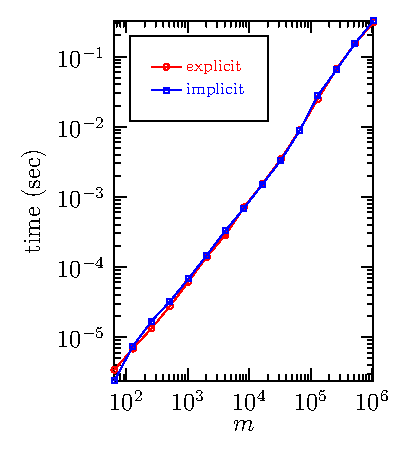
\includegraphics{timing1c}
\caption{Comparison of computation times for explicitly and implicitly
dealiased complex in-place 1D convolutions of two vectors of
(unpadded) length $m$. The storage requirements of the two algorithms are
identical.}
\label{timing1c}
\end{center}
\end{minipage}
\end{figure}

Referring to the computation times shown in Figure~\ref{timing1c},
we see that the implicit padding algorithm described by \Eqs{cconv1backwards} 
and~\hEq{cconv1forwards}
can be implemented to be quite competitive with an explicitly padded
convolution. Both the FFTW library and the convolution layer we built on
top of it were compiled with the Intel C/C++ compiler, using
the same optimization options, on a 64-bit 3GHz Intel E5450 Xenon processor
with 6MB cache. Like the FFTW library, our algorithm was vectorized with
specialized single-instruction multiple-data (SIMD) code. 

\subsection{Implicitly dealiased centered Fourier transform}\label{fft0}
A basic building block for constructing multidimensional pseudospectral
convolutions is an implicitly dealiased centered Fourier transform, where the
input data length is odd, say $2m-1$, with the Fourier origin at index $m-1$. 
Here, one needs to pad to $N\ge 3m-2$ to prevent 
mode $m-1$ from beating with itself to contaminate the most negative
(first) mode, at wavenumber $-m+1$. Since the ratio of the number of physical to
total modes, $(2m-1)/(3m-2)$ is asymptotic to $2/3$ for large $m$, this
padding scheme is often referred to as the {\it $2/3$ padding rule}.

For explicit padding, one usually chooses the padded vector length
$N$ to be a power of $2$, with $m=\floor{(n+2)/3}$. However, for implicit
padding, it is advantageous to choose $m$ itself to be a power of $2$
since the algorithm reduces to computing FFTs of length $m$.
Moreover, it is convenient to pad implicitly slightly beyond $3m-2$, to $N=3m$,
as this allow the use of a radix $3$ subdivision at the highest level, so
that only two of the three subtransforms of length $m$ need to be retained. 

Suppose then that $U_k=0$ for $k\ge m$.
On decomposing $j=(3\ell+r)\mod N$, where $r\in\{-1,0,1\}$, the 
substitution $k'=m+k$ allows us to write the backwards transform as
\bel
u_{3\ell +r}\no=\sum_{k=-m+1}^{m-1}\z_m^{\ell k} \z_N^{rk} U_k
=\sum_{k'=1}^{m-1}\z_m^{\ell k'} \z_N^{r(k'-m)} U_{k'-m}
+\sum_{k=0}^{m-1}\z_m^{\ell k} \z_N^{rk} U_k
=\sum_{k=0}^{m-1}\z_m^{\ell k} w_{k,r},\label{fft0backwardsA}
\eel
where
\bel
w_{k,r}\doteq
\cases{
U_0&if $k=0$,\cr
\z_N^{rk}(U_k+\z_3^{-r}U_{k-m})&if $1\le k\le m-1$.\cr
}\label{fft0backwardsB}
\eel
The forwards transform is then
\bel
NU_k=\sum_{r=-1}^{1}\zeta_N^{-rk}\sum_{\ell=0}^{m-1}\zeta_m^{-\ell k} u_{3\ell+r}
\qquad k\no =-m+1,\ldots,m-1.\label{fft0forwards}
\eel
The use of the remainder $r=-1$ instead of $r=2$ allows us to exploit
the optimization $\zeta_N^{-k}=\conj{\zeta_N^ k}$ in \Eqs{fft0backwardsB}
and~\hEq{fft0forwards}.
The number of complex multiplies needed to evaluate \Eq{fft0backwardsB} 
for $r=\pm 1$ can be reduced by computing the intermediate complex quantities
\bg
\be
A_k\doteq \zeta_N^k\(\Re U_k+\zeta_3^{-1} \Re U_{k-m}\),
\ee
\be
B_k\doteq i\zeta_N^k\(\Im U_k+\zeta_3^{-1} \Im U_{k-m}\),
\ee
\eg
where $\zeta_3^{-1}=\(-\half,-\fr{\sqrt{3}}{2}\)$, so that for $k > 0$,
$w_{k,1}=A_k+B_k$ and $w_{k,-1}=\conj{A_k-B_k}$.
The resulting transforms,
Procedures \ref{fft0padBackwards} and \ref{fft0padForwards},
each have an operation count asymptotic to $3Km\log m$. As they
operate fully in place on their arguments, with no additional storage
requirements, it is straightforward to implement strided multivector
versions of these routines.

\begin{procedure}[htbp]
  \KwIn{vector \xf}
  \KwOut{vector \xf, vector \xu}
  $\xu[0] \leftarrow \xf[m-1]$\;
  \For{$k=1$ \KwTo $m-1$}{
    $\xA \leftarrow \zeta_{3m}^k*\[\Re \xf[m-1+k]+\(-\half,-\fr{\sqrt{3}}{2}\)*\Re \xf[k]\]$\;
    $\xB \leftarrow i\zeta_{3m}^k*\[\Im \xf[m-1+k]+\(-\half,-\fr{\sqrt{3}}{2}\)*\Im \xf[k]\]$\;
    $\xf[m-1+k] \leftarrow \xA+\xB$\;
    $\xu[k] \leftarrow \conj{\xA-\xB}$\;
    $\xf[0] \leftarrow \xf[k]$\;
    $\xf[k] \leftarrow \xf[k]+\xf[m-1+k]$\;
  }

  $\xf[0,\ldots,m-1] \leftarrow {\tt fft}\inv(\xf[0,\ldots,m-1])$\;
  $\xu[m] \leftarrow \xf[m-1]$\;
  $\xf[m-1] \leftarrow \xu[0]$\;
  $\xf[m-1,\ldots,2m-2] \leftarrow {\tt fft}\inv(\xf[m-1,\ldots,2m-2])$\;
  $\xu[0,\ldots,m-1] \leftarrow {\tt fft}\inv(\xu[0,\ldots,m-1])$\;
  \caption{fft0padBackwards(vector {\sf f}, vector {\sf u}) stores the scrambled
$3m$-padded centered backwards Fourier transform values of a vector {\sf f} of length
$2m-1$ in {\sf f} and an auxiliary vector~{\sf u} of length $m+1$.}\label{fft0padBackwards}
\end{procedure}

\begin{function}[htbp]
  \KwIn{vector \xf, vector \xu}
  \KwOut{vector \xf}

  $\xf[m-1,\ldots,2m-2] \leftarrow {\tt fft}(\xf[m-1,\ldots,2m-2])$\;
  $\xu[m] \leftrightarrow \xf[m-1]$\;

  $\xf[0,\ldots,m-1] \leftarrow {\tt fft}(\xf[0,\ldots,m-1])$\;
  $\xu[0,\ldots,m-1] \leftarrow {\tt fft}(\xu[0,\ldots,m-1])$\;

  $\xu[m] \leftarrow \xf[0]+\xu[m]+\xu[0]$\;
  \For{$k=1$ \KwTo $m-1$}{
    $\xf[k-1]=\xf[k]+\(-\half,\fr{\sqrt{3}}{2}\)*\zeta_{3m}^{-k}*\xf[m-1+k]+\(-\half,-\fr{\sqrt{3}}{2}\)*\zeta_{3m}^k*\xu[k]$\;
    $\xf[m-1+k]=\xf[k]+\zeta_{3m}^{-k}*\xf[m-1+k]+\zeta_{3m}^k*\xu[k]$\;
  }
  $\xf[m-1] \leftarrow \xu[m]$\;
  \Return \xf/(3m)\;
  \caption{fft0padForwards(vector {\sf f}, vector {\sf u}) returns the
inverse of fft0padBackwards(vector {\sf f}, vector {\sf u}).}
\label{fft0padForwards}
\end{function}

\subsection{Hermitian convolution}

In this frequently encountered case (relevant to the pseudospectral
method), each input vector is the Fourier transform of real-valued data;
that is, it satisfies the {\it Hermiticity condition} $U_{-k}=\conj{U_k}$.
While the physical data represented is of length $2m-1$, centered
about the Fourier origin, the redundant negative wavenumbers are not
included in the input vectors. The input vectors are thus of length $m$,
with the Fourier origin at index $0$. Just as in Section~\ref{fft0},
the unsymmetrized physical data needs to be padded with at least $m-1$ zeros.
Hermitian symmetry then requires us to pad the $m$ non-negative
wavenumbers with at least $c\doteq\floor{m/2}$ zeros.
The resulting $2/3$ padding ratio (for even $m$) turns out to work
particularly well for developing implicitly dealiased Hermitian convolutions.
As in the centered case, we again choose the Fourier size to be $N=3m$.

Given that $U_k=0$ for $k\ge m$, the backwards (complex-to-real) transform
appears as \Eq{fft0backwardsA}, but now with
\bel
w_{k,r}\doteq
\cases{
U_0&if $k=0$,\cr
\z_N^{rk}\(U_k+\z_3^{-r}\conj{U_{m-k}}\)&if $1\le k\le m-1$.\cr
}
\eel

We note that $w_{k,r}$ obeys the Hermitian symmetry 
$w_{k,r}=\conj{w_{m-k,r}}$, so that the Fourier transform
$\sum_{k=0}^{m-1}\z_m^{\ell k} w_{k,r}$ in \Eq{fft0backwardsA} will indeed
be real valued. This allows us to build a backwards implicitly dealiased
Hermitian transform using three complex-to-real Fourier transforms of the
first $c+1$ components of $w_{k,r}$ (one for each $r\in\{-1,0,1\}$). The
forwards transform is given by
\bel
NU_k
=\sum_{r=-1}^{1}\zeta_N^{-rk}\sum_{\ell=0}^{m-1}\zeta_m^{-\ell k} u_{3\ell+r}
\qquad k\no =0,\ldots,m-1.\label{fft0forwardsB}
\eel
Since $u_{3\ell+r}$ is real, a real-to-complex transform can be used to
compute the first $c+1$ frequencies of
$\sum_{\ell=0}^{m-1}\zeta_m^{-\ell k} u_{3\ell+r}$; the remaining $m-c-1$
frequencies needed in \Eq{fft0forwardsB} are then computed using Hermitian
symmetry. Since there are two input vectors and
one output vector, the complete convolution requires a total of nine
Hermitian Fourier transforms of size $m$, for an overall computational
scaling of $\fr{9}{2}K m \log m$ operations, in agreement with the
leading-order scaling of an explicitly padded centered Hermitian convolution.
We see in Function~\ref{conv} that seven out of these nine Fourier
transforms can be performed out of place using the same amount of memory,
$2(N/2+1)=6c+2$, as would be used to compute a centered Hermitian convolution with
explicit padding.

For simplicity, we first consider the case where $m=2c$.
To facilitate an in-place implementation of the backwards transform, we
store the conjugate of the transformed values for $r=1$ in reverse order in
the upper half of the $f$ vector, using the identity (for real $u_j$)
$$
u_j=\conj{u_j}=\sum_{k=-c+1}^{c}\zeta_m^{-jk} \conj{U_k}
=\sum_{k'=m-1}^{0}\zeta_m^{j(k'-c)} \conj{U_{c-k'}}
=(-1)^j\sum_{k=0}^{m-1}\zeta_m^{jk} \conj{U_{c-k}}
$$
obtained using the substitution $k'=c-k$. One can omit the factors of
$(-1)^j$ since they will cancel during the real term-by-term multiplication
of the two transformed input vectors.

\begin{function}[htbp]
  \SetKwFunction{build}{build}
  \KwIn{vector \xf, vector \xg}
  \KwOut{vector \xf}
  $\xF \leftarrow \xf[c]$\;
  $\xG \leftarrow \xg[c]$\;
  \medskip
  \build{\xf,\xu}\;
  \build{\xg,\xv}\;
  \medskip
  $\xC \leftarrow \xf[c]$\;
  $\xf[c] \leftarrow 2\Re \xF$\;
  $\xu[c] \leftarrow \Re \xF+\sqrt{3}\Im \xF$\;
  \medskip
  $\xD \leftarrow \xg[c]$\;
  $\xg[c] \leftarrow 2\Re \xG$\;
  $\xv[c] \leftarrow \Re \xG+\sqrt{3}\Im \xG$\;
  \medskip
  $\xu \leftarrow \crfft(\xu)$\;
  $\xv \leftarrow \crfft(\xv)$\;
  $\xv \leftarrow \xv * \xu$\;
  $\xu \leftarrow \rcfft(\xv)$\;
  \medskip
  $\xv \leftarrow \crfft(\xf[0,\ldots,c])$\;
  $\xf[0,\ldots,c] \leftarrow \crfft(\xg[0,\ldots,c])$\;
  $\xv \leftarrow \xv * \xf[0,\ldots,c]$\;
  $\xf[0,\ldots,c] \leftarrow \rcfft(\xv)$\;
  \medskip
  $\xS\leftarrow \xf[c-1]$\;
  $\xT\leftarrow \xf[c]$\;
  $\xf[c-1]=\Re \xF-\sqrt{3}\Im \xF$\;
  $\xf[c]=\xC$\;
  $\xg[c-1]=\Re \xG-\sqrt{3}\Im \xG$\;
  $\xg[c]=\xD$\;
  \medskip
  $\xv \leftarrow \crfft(\xg[c-1,\ldots,2c-1])$\;
  $\xg[c-1,\ldots,2c-1] \leftarrow \crfft(\xf[c-1,\ldots,2c-1])$\;
  $\xg[c-1,\ldots,2c-1] \leftarrow \xg[c-1,\ldots,2c-1] * \xv$\;
  $\xv\leftarrow \rcfft(\xg[c-1,\ldots,2c-1])$\;
  \medskip

  \For{$k=1$ \KwTo $c-2$}{
    $\xf[k]=\xf[k]+\zeta_{6c}^{-k}*\xv[k]+\zeta_{6c}^k*\xu[k]$\;
    $\xf[2c-k]=\conj{\xf[k]}+\(-\half,-\fr{\sqrt{3}}{2}\)*\zeta_{6c}^k*\conj{\xv[k]}+\(-\half,\fr{\sqrt{3}}{2}\)*\zeta_{6c}^{-k}*\conj{\xu[k]}$\;
  }

  $\xf[c-1]=S+\zeta_{6c}^{1-c}*\xv[c-1]+\zeta_{6c}^{c-1}*\xu[c-1]$\;
  $\xf[c]=T-\(-\half,\fr{\sqrt{3}}{2}\)*\xv[c]-\(-\half,-\fr{\sqrt{3}}{2}\)*\xu[c]$\;
  $\xf[c+1]=\conj{S}+\(-\half,-\fr{\sqrt{3}}{2}\)*\zeta_{6c}^{c-1}*\conj{\xv[c-1]}+\(-\half,\fr{\sqrt{3}}{2}\)*\zeta_{6c}^{1-c}*\conj{\xu[c-1]}$\;

  \Return f/(6c)\;
\caption{conv(vector {\sf f}, vector {\sf g}) 
uses Procedure~\ref{build} to compute
an in-place implicitly dealiased convolution of centered Hermitian vectors
{\sf f} and {\sf g} of length~$2c$ using temporary vectors {\sf u} and
{\sf v} of length $c+1$.}\label{conv}
\end{function}

\begin{figure}[htbp]
\begin{minipage}{0.5\linewidth}
\begin{procedure}[H]
  \KwIn{vector \xf}
  \KwOut{vector \xf, vector \xu}
  $\xu[0] \leftarrow \xf[0]$\;
  $\xFk \leftarrow \conj{f[m-1]}$\;
  $\xf[m-1] \leftarrow \xf[0]$\;
  \For{$k=1$ \KwTo $c-1$}{
    $\xA \leftarrow \zeta_{6c}^k*\phantom{\quad}
\[\Re \xf[k]+\(-\half,\fr{\sqrt{3}}{2}\)*\Re \xFk\]$\;
    $\xB \leftarrow -i\zeta_{6c}^k*\phantom{\quad}
\[\Im \xf[k]+\(-\half,\fr{\sqrt{3}}{2}\)*\Im \xFk\]$\;
    $\xf[k] \leftarrow \xf[k]+\xFk$\;
    $\xu[k] \leftarrow \xA-\xB$\;
    $\xFk \leftarrow \conj{\xf[m-1-k]}$\;
    $\xf[m-1-k] \leftarrow \xA+\xB$\;
  }
  \caption{build(vector~{\sf f}, vector~{\sf u}) builds the FFT arrays
required for Procedure~\ref{conv} from an unpadded vector {\sf f} of length
$2c$ into {\sf f} and an auxiliary vector~{\sf u} of length
$c+1$.}\label{build}
\end{procedure}
\end{minipage}
\begin{minipage}{0.5\linewidth}
\begin{center}
%On orcinus, using N=100000000.
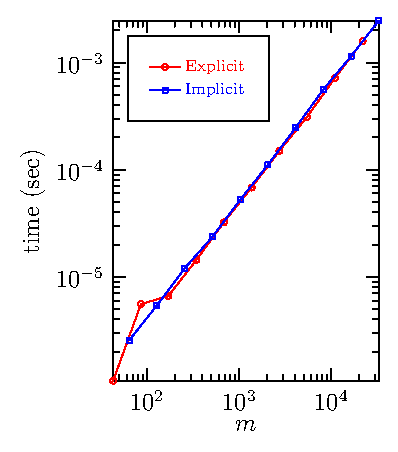
\includegraphics{timing1r}
\caption{Comparison of computation times for explicitly and implicitly
dealiased centered Hermitian in-place 1D convolutions of two vectors of
(unpadded) length $(2m-1)$.}
\label{timing1r}
\end{center}
\end{minipage}
\end{figure}


\begin{comment}
$$
u_j=\sum_{k=0}^{N-1}\zeta_N^{jk} U_k
=\sum_{k=0}^{2m-1}\zeta_N^{jk} U_k
$$
Then 
\bel
u_{3\ell}= \sum_{k=0}^{2m-1}\z_{3m}^{3\ell k} U_k
=\sum_{k=0}^{m-1}\z_m^{\ell k} U_k
+\sum_{k=m}^{2m-1}\z_m^{\ell k} U_k
=\sum_{k=0}^{m-1}\z_m^{\ell k} U_k
+\sum_{k=0}^{m-1}\z_m^{\ell (k+m)} U_{k+m}
=\sum_{k=0}^{m-1}\z_m^{\ell k} \(U_k+U_{k+m}\).\label{DFTm}
\eel
Equation~\ref{DFTm} is a DFT of length $m$,
each requiring $m\log m$ operations. Following a similar procedure,
with $r=1$ or $r=2$,
\bel
\label{dfft23g}
u_{3\ell +r}\no=
 \sum_{k=0}^{m-1}\z_m^{\ell k} \(\z_N^{rk} U_k + \z_N^{r(k+m)}U_{k+m}\)
\eel
The forward Fourier transform appears as
\be
NU_k=\sum_{j=0}^{N-1}\zeta_N^{-kj} u_j
=\sum_{r=0}^{2}\zeta_N^{-rk}\sum_{\ell=0}^{m-1}\zeta_N^{-3\ell k} u_{3\ell+r}
=\sum_{r=0}^{2}\zeta_N^{-rk}\sum_{\ell=0}^{m-1}\zeta_m^{-\ell k} u_{3\ell+r}
\qquad k\no =0,\ldots,pm-1.
\ee
\end{comment}

The computation times for a implicitly dealiased Hermitian
convolution are compared with those for an explicitly padded convolution in
Figure~\ref{timing1r}. For the intended application to partial differential
equations, there is flexibility in the choice of the exact convolution
size. This is why we consider for each algorithm only those vector lengths
that maximize performance.

On the other hand, for those applications where the size of the convolution
is dictated by external criteria, implicit padding effectively expands the
available set of efficient convolutions sizes to include integral powers of
$2$, a case of practical significance. The existence of implicit convolutions in
fact nullifies the argument of Canuto...
% Address slightly misleading implication of Canuto page 136
% (dealiased.pdf: p.20) regarding power of 2 transforms (depends on
% application).

\section{Implicitly dealiased 2D convolutions}\label{2d}

\subsection{Complex 2D convolution}
The algorithms developed in the previous sections can be used as building
blocks to construct the efficient implicitly padded 2D convolution shown in
Algorithm~\ref{cconv2}. As shown in Figure~\ref{timing2c}, the implicit
algorithm now outperforms the explicit version. 
For example, a $1024\times 1024$ complex convolution runs $48\%$ faster
than an explicit convolution. The gains appear to increase with transform
size: a $8192\times 8192$ implicit convolution runs $52\%$ faster than an
explicit one.

The third sentence of the quote from Steven G. Johnson
on page~\ref{quote} suggests a very reasonable optimization
for explicitly padded 2D convolutions.
However there are other optimization possibilities lost in directly
expressing a 2D convolution in terms of 1D transforms: as illustrated in
Figure~\ref{cconv2}, while the $y$-pruned explicit convolution is 27\% faster
than a conventional 2D explicit convolution for size $1024\times 1024$ but
$71\%$ slower for a $8192\times 8192$ convolution. Our implicitly dealised
convolution is also subject to these same losses, but the savings due to
implicit padding, ignoring high-level bit reversal, in-place subtransforms, 
and computing the convolution of each column as it is transformed (and
thereby perhaps still in cache) outweighs these losses.
%CHECK timing again when using mfft in both directions for pruned algorithm.

Because the same temporary arrays $u$ and $v$ are used for each column
of the convolution, the memory requirements are $4m_xm_y+2m_y$ complex
words in comparison to the $8m_xm_y$ complex words required for an
explicitly padded convolution. Asymptotically, as $m_x\goesto\infty$,
a 2D implicit complex convolution therefore requires half the memory
required by zero padding.

%Discuss proper storage direction & use of multiple ffts.

\subsection{Centered 2D Hermitian convolution}

In two dimensions, the Fourier-centered Hermiticity condition appears as
$U_{-k,-\ell}=\conj{U_{k,\ell}}$. 
This symmetry is exploited in the centered Hermitian convolution
algorithm described in Function~\ref{conv2}. As shown in
Figure~\ref{timing2c}, one again observes a dramatic improvement in speed.

When $m$ is even, the memory usage for a $(2m-1)\times (2m-1)$ Hermitian
convolution is $2(2m-1)m+2(m+1)m+2(m/2+1)=6m^2+m+2$ complex words,
compared with a minimum of $2(3m-2)(3m/2)=9m^2-6m$ complex words for an explicit
transform.

\begin{figure}[htbp]
\begin{minipage}{0.49\linewidth}
\begin{function}[H]
  \KwIn{matrix \xf, matrix \xg}
  \KwOut{matrix \xf}
  \For{$j=0$ \KwTo $m_y-1$}{
    $\fftpadBackwards(\xf^T[j],\xU^T[j])$\;
    $\fftpadBackwards(\xg^T[j],\xV^T[j])$\;
  }
  \For{$i=0$ \KwTo $m_x-1$}{
    $\cconv(\xf[i],\xg[i],\xu,\xv)$\;
    $\cconv(\xU[i],\xV[i],\xu,\xv)$\;
  }
  \For{$j=0$ \KwTo $m_y-1$}{
    $\fftpadForwards(\xf^T[j],\xU^T[j])$\;
  }
  \Return \xf\;
\caption{cconv2(matrix~{\sf f}, matrix~{\sf g}) 
returns an in-place implicitly dealiased convolution of
$m_x\times m_y$ matrices {\sf f} and {\sf g} using temporary $m_x\times m_y$
matrices {\sf U} and {\sf V} and temporary vectors {\sf u} and {\sf v} of
length $m_y$.}\label{cconv2}
\end{function}
\end{minipage}
\begin{minipage}{0.51\linewidth}
\begin{function}[H]
  \KwIn{matrix \xf, matrix \xg}
  \KwOut{matrix \xf}
  \For{$j=0$ \KwTo $m_y-1$}{
    $\fftOpadBackwards(\xf^T[j],\xU^T[j])$\;
    $\fftOpadBackwards(\xg^T[j],\xV^T[j])$\;
  }
  \For{$i=0$ \KwTo $2m_x-2$}{
    $\conv(\xf[i],\xg[i],\xu,\xv)$\;
  }
  \For{$i=0$ \KwTo $m_x$}{
    $\conv(\xU[i],\xV[i],\xu,\xv)$\;
  }
  \For{$j=0$ \KwTo $m_y-1$}{
    $\fftOpadForwards(\xf^T[j],\xU^T[j])$\;
  }
  \Return \xf\;
\caption{conv2(matrix~{\sf f}, matrix~{\sf g}) 
returns an in-place implicitly dealiased convolution of $(2m_x-1)\times
m_y$ matrices {\sf f} and {\sf g} using temporary $(m_x+1)\times m_y$ matrices 
{\sf U} and {\sf V} and temporary vectors {\sf u} and {\sf v} of length $m_y$.
}\label{conv2}
\end{function}
\end{minipage}
\end{figure}

\begin{figure}[htbp]
\begin{center}
\begin{minipage}{0.49\linewidth}
\begin{center}
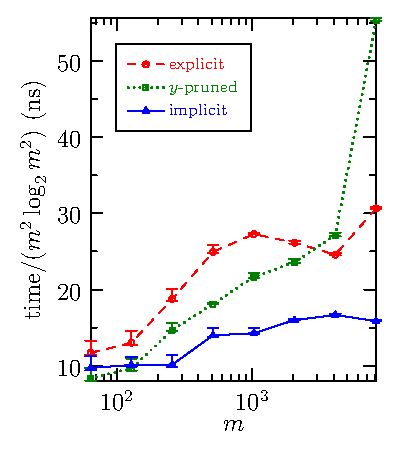
\includegraphics{timing2c}
\caption{Comparison of computation times for explicitly and implicitly
dealiased complex in-place 2D convolutions of two matrices of
(unpadded) length $m\times m$.}
\label{timing2c}
\end{center}
\end{minipage}
%
\begin{minipage}{0.49\linewidth}
\begin{center}
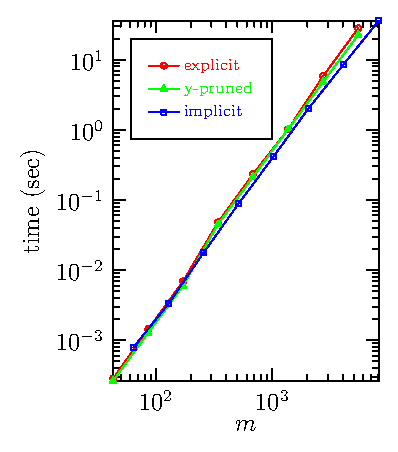
\includegraphics{timing2r}
\caption{Comparison of computation times for explicitly and implicitly
dealiased centered Hermitian in-place 2D convolutions of two matrices of
(unpadded) length $(2m-1)\times m$.}
\label{timing2r}
\end{center}
\end{minipage}
\end{center}
\end{figure}

%TODO: Improve, show column convolutions, strides, dimensions, padding,
%etc.  Also make a 3D version.
\begin{figure}[htbp]
  \begin{center}
    \includegraphics{dealias2d}
    \caption{Two-dimensional convolution procedure.}
    \label{dealias2d}
  \end{center}
\end{figure}

\section{Implicitly dealiased 3D convolutions}\label{3d}

\section{Implicitly dealiased biconvolutions}\label{hyper}

\subsection{Implicitly double dealiased centered Fourier transform}
\label{fft0bi}
Implicit padding is well-suited to dealiasing the centered biconvolution 
$$
\sum_{p=-m+1}^{m-1}\sum_{q=-m+1}^{m-1}\sum_{r=-m+1}^{m-1} f_p g_q h_r\d_{p+q+r,k}.
$$
Here the input data length is $2m-1$, with the Fourier origin at index
$m-1$, so one needs to pad to $N\ge 4m-3$ to prevent contamination due to
wave beating.

Implicit padding is most efficiently implemented by padding the input
vector with a single zero complex word at the beginning, to yield a vector
of length $2m$, with the Fourier origin at index $m$. We choose $m$ to be
a power of $2$ and $N=4m$. Here, $U_k=0$ for $k=0$ and $k\ge m$. 

On decomposing $j=2\ell+r$, where $\ell=0,\ldots, 2m-1$ and $r\in\{0,1\}$,
we find on substituting $k'=k+m$ that
\bel
u_{2\ell +r}\no=\sum_{k=-m}^{m-1}\z_{2m}^{\ell k} \z_N^{rk} U_k
=\sum_{k'=0}^{2m-1}\z_{2m}^{\ell (k'-m)} \z_N^{r(k'-m)} U_{k'-m}
=(-1)^\ell i^{-r}\sum_{k=0}^{2m-1}\z_{2m}^{\ell k} \z_N^{rk} U_{k-m}.
\label{fft0bibackwards}
\eel
The scaled forwards transform is then given by
\bel
NU_k=\sum_{r=0}^{1}\zeta_N^{-rk}\sum_{\ell=0}^{2m-1}\zeta_{2m}^{-\ell k} u_{2\ell+r},
\qquad k\no =-m+1,\ldots,m-1
=\sum_{r=0}^{1}\zeta_N^{-r(k'-m)}\sum_{\ell=0}^{2m-1}\zeta_{2m}^{-\ell (k'-m)} u_{2\ell+r},
=\sum_{r=0}^{1}\zeta_N^{-rk'}i^r\sum_{\ell=0}^{2m-1}\zeta_{2m}^{-\ell k'}(-1)^\ell u_{2\ell+r},
\qquad k'\no =1,\ldots,2m-1.\label{fft0biforwards}
\eel
For a biconvolution, the product of the three factors $(-1)^\ell$
(one for each input vector) arising from \Eq{fft0bibackwards}
and the factor $(-1)^\ell$ in \Eq{fft0biforwards} cancel.
Procedures \ref{fft0bipadBackwards} and \ref{fft0bipadForwards},
each have an operation count asymptotic to $4Km\log m$. As they
operate fully in place on their arguments, with no additional storage
requirements, it is straightforward to implement strided multivector
versions of these routines.

\subsection{Implicitly dealiased centered Hermitian 1D biconvolution}
Let us now consider a Hermitian biconvolution with $N=4m$, where $m$ is a
power of $2$. For explicit padding, one needs to pad the $m$ non-negative
wavenumbers with $m+1$ zeros, for a total vector length of $2m+1$.

On decomposing $j=2\ell+r$, where
$\ell=0,\ldots, 2m-1$ and $r\in\{0,1\}$, the backwards transform is given
by
\bec
u_{2\ell +r}=\sum_{k=-m}^{m-1} \z_{2m}^{\ell k} \z_N^{rk} U_k.
\eec
If we set $U_m=0$, the real components $u_{2\ell +r}$ can thus be computed
by taking a complex-to-real $2m$ transform of
$\{\z_N^{rk} U_k : k=0,\ldots m\}$.

The forwards transform is
\be
NU_k=\sum_{r=0}^{1}\zeta_N^{-rk}
\sum_{\ell=0}^{2m-1} \zeta_{2m}^{-\ell k} u_{2\ell+r}
\qquad k\no =-m+1,\ldots,m-1.
\ee

The resulting implicitly padded Hermitian biconvolution,
Procedure \ref{biconv}, has an operation count of $8Km\log m$. In
Fig.~\ref{timing1b} we show that this algorithm is competitive with
explicit padding. Explicit padding requires $3(2m+1)=6m+3$ complex words,
whereas implicit padding requires $6(m+1)$ complex words of storage.

\begin{figure}[htbp]
\begin{minipage}{0.51\linewidth}
\begin{procedure}[H]
  \KwIn{vector \xf}
  \KwOut{vector \xf, vector \xu}
  $\xu[0]=\xf[0]=0$\;
  \For{$k=1$ \KwTo $2m-1$}{
    $\xu[k] \leftarrow -i\z_{4m}^k * \xf[k]$\;
  }
  $\xf \leftarrow \fft\inv(\xf)$\;
  $\xu \leftarrow \fft\inv(\xu)$\;
  \Return f;
  \caption{fft0bipadBackwards(vector~{\sf f}, vector~{\sf u}) stores the 
scrambled signed~$4m$-padded centered backwards Fourier transform values of a
vector {\sf f} of length~$2m$ in {\sf f} and an auxiliary vector~{\sf u} of
length $2m$.}\label{fft0bipadBackwards}
\end{procedure}
\end{minipage}
\begin{minipage}{0.49\linewidth}
\begin{function}[H]
  \KwIn{vector \xf, vector \xu}
  \KwOut{vector \xf}
  $\xf \leftarrow \fft(\xf)$\;
  $\xu \leftarrow \fft(\xu)$\;
  \For{$k=1$ \KwTo $2m-1$}{
    $\xf[k] \leftarrow \xf[k] +i \z_{4m}^{-k} * \xu[k]$\;
  }
  \Return \xf/(4m)\;
  \caption{fft0bipadForwards(vector~{\sf f}, vector~{\sf u}) returns the
inverse of fft0bipadBackwards(\hbox{vector~{\sf f}, vector~{\sf u}}).}
\label{fft0bipadForwards}
\end{function}
\end{minipage}
\end{figure}

Just as for convolutions, the performance and memory benefits of
evaluating implicitly padded hyperconvolutions manifest themselves only in
higher dimensions. For example, in Figure~\ref{timing2b}, we observe 
that an implicit $8192\times 8192$ Hermitian biconvolution requires $46\%$
of the computation time required for an explicit biconvolution.
The memory usage for a $(2m-1)\times (2m-1)$ Hermitian biconvolution
is $6\cdot 2m(m+1)+3(m+1)=12m^2+15m+1$ complex words, compared with
$3\cdot 4m(2m+1)=24m^2+12m$ complex words for an explicit power-of-two
transform. For small sizes, $y$-pruned biconvolutions appear to be
faster than the other two algorithms, while for large sizes implicit
padding is best. For example, an $8192\times 8192$ $y$-pruned biconvolution
requires $63\%$ of the computation time and the same amount of storage as
an explicitly padded biconvolution.

\begin{figure}[htbp]
\begin{minipage}{0.445\linewidth}
\begin{function}[H]
  \KwIn{vector \xf, vector \xg, vector \xh}
  \KwOut{vector \xf}
  \For{$k=0$ \KwTo $m-1$}{
    $\xu[k] \leftarrow \z_{4m}^k * \xf[k]$\;
    $\xv[k] \leftarrow \z_{4m}^k * \xg[k]$\;
    $\xw[k] \leftarrow \z_{4m}^k * \xh[k]$\;
  }
  \medskip
  $\xu[m]=\xv[m]=\xw[m]=0$\;
  $\xu \leftarrow \crfft\inv(\xu)$\;
  $\xv \leftarrow \crfft\inv(\xv)$\;
  $\xw \leftarrow \crfft\inv(\xw)$\;
  $\xv \leftarrow \xu * \xv * \xw$\;
  $\xu \leftarrow \rcfft(\xv)$\;
  \medskip
  $\xf[m]=\xg[m]=\xh[m]=0$\;
  $\xv \leftarrow \crfft\inv(\xf)$\;
  $\xf \leftarrow \crfft\inv(\xg)$\;
  $\xg \leftarrow \crfft\inv(\xh)$\;
  $\xv \leftarrow \xv * \xf * \xg$\;
  $\xf \leftarrow \rcfft(\xv)$\;
  \medskip
  \For{$k=0$ \KwTo $m-1$}{
    $\xf[k] \leftarrow \xf[k] + \z_{4m}^{-k} * \xu[k]$\;
  }
  \Return f/(4m)\;
\caption{biconv(vector {\sf f}, vector~{\sf g}, vector~{\sf h}) computes
an in-place implicitly dealiased biconvolution of three centered
Hermitian vectors {\sf f}, {\sf g}, {\sf h}, using three temporary vectors
{\sf u}, {\sf v}, and {\sf w}, each of length~$m+1$.}\label{biconv}
\end{function}
\end{minipage}
\begin{minipage}{0.545\linewidth}
\begin{function}[H]
  \KwIn{matrix \xf, matrix \xg, matrix \xh}
  \KwOut{matrix \xf}
  \For{$j=0$ \KwTo $m_y-1$}{
    $\fftObipadBackwards(\xf^T[j],\xU^T[j])$\;
    $\fftObipadBackwards(\xg^T[j],\xV^T[j])$\;
    $\fftObipadBackwards(\xh^T[j],\xW^T[j])$\;
  }
  \For{$i=0$ \KwTo $2m_x-1$}{
    $\biconv(\xf[i],\xg[i],\xh[i],\xu,\xv,\xw)$\;
    $\biconv(\xU[i],\xV[i],\xW[i],\xu,\xv,\xw)$\;
  }
  \For{$j=0$ \KwTo $m_y-1$}{
    $\fftObipadForwards(\xf^T[j],\xU^T[j])$\;
  }
  \Return \xf\;
\caption{biconv2(matrix~{\sf f}, matrix~{\sf g}, matrix~{\sf h}) 
returns an in-place implicitly dealiased convolution of \hbox{$2m_x\times
(m_y+1)$} matrices~{\sf f},~{\sf g}, and~{\sf h} using
temporary \hbox{$2m_x\times (m_y+1)$} matrices~{\sf U}, {\sf V}, and~{\sf W} and
temporary vectors {\sf u}, {\sf v} and~{\sf w} of length~$m_y+1$.
}\label{biconv2}
\end{function}
\end{minipage}
\end{figure}

\begin{figure}[htbp]
\begin{center}
\begin{minipage}{0.49\linewidth}
\begin{center}
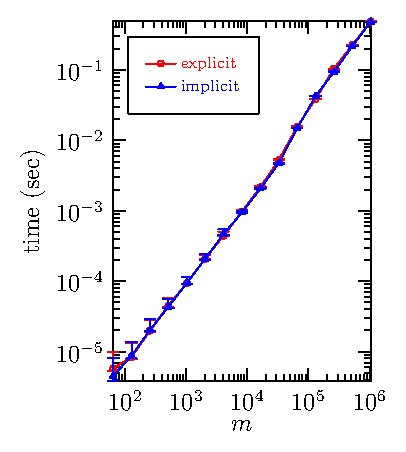
\includegraphics{timing1b}
\caption{Comparison of computation times for explicitly and implicitly
dealiased complex in-place 1D biconvolutions of two vectors of
(unpadded) length $m$.}
\label{timing1b}
\end{center}
\end{minipage}
%
\begin{minipage}{0.49\linewidth}
\begin{center}
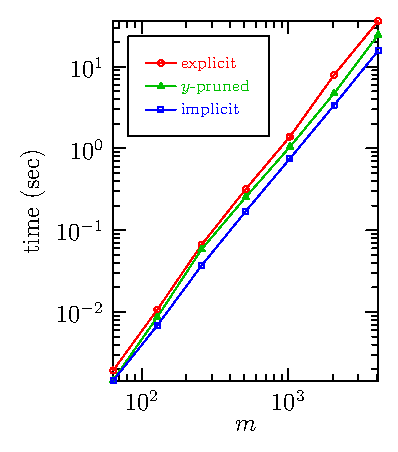
\includegraphics{timing2b}
\caption{Comparison of computation times for explicitly and implicitly
dealiased centered Hermitian in-place 2D biconvolutions of two matrices of
(unpadded) size $(2m-1)\times m$.}
\label{timing2b}
\end{center}
\end{minipage}
\end{center}
\end{figure}

\section{Arbitrary $p/q$ Padding}

In general, consider a ``$p/q$'' padding in which $N=qm$, and only $pm$ modes
are non-zero, with $p$ and $q$ relatively prime. Consider $u_{q\ell+r}$, with
$\ell=0 \dots m-1$, $r=0 \dots q-1$.
Then
\be
u_{q\ell+r} = \sum_{k=0}^{N-1}\z_N^{(q\ell+r)k} U_k
= \sum_{k=0}^{pm-1}\z_{qm}^{(q\ell+r)k} U_k
= \sum_{k=0}^{pm-1}\z_m^{\ell k}\z_{N}^{rk} U_k
= \sum_{\a=0}^{p-1} \sum_{k=\a m}^{(\a+1)m-1}\z_m^{\ell k}\z_{N}^{rk} U_k
= \sum_{\a=0}^{p-1} \sum_{\k=0}^{m-1}\z_m^{\ell (\k+\a m)}\z_{N}^{r(\k+\a m)}
U_{\k+\a m}
%=  \sum_{\a=0}^{p-1}\z_N^{r \a m} \sum_{\k=0}^{m-1}\z_m^{\ell\k}\z_N^{r\k}U_{\k+\a m}
=  \sum_{\k=0}^{m-1}\z_m^{\ell\k}\sum_{\a=0}^{p-1}\z_N^{r(\k+\a m)} U_{\k+\a m}
\ee .
Note that, in the last line, we have the choice of which $\z$ to use, since
$\z_q^{r \a}=\z_N^{r \a m}$. Since there are $m$ choices of $r$ and $q$ choices
for $\ell$, we are left with $mq=N$ FFTs of length $p$, leaving on the order
of $N \log p = N \log (N/q)$ operations.  Again, while the computational
savings is only marginal, this formulation affords significant improvements
in memory use and parallelizability.

The forward Fourier transform appears as
\be
NU_k=\sum_{j=0}^{N-1}\zeta_N^{-kj} u_j
=\sum_{r=0}^{q-1}\zeta_N^{-rk}\sum_{\ell=0}^{m-1}\zeta_N^{-q\ell k} u_{q\ell+r}
=\sum_{r=0}^{q-1}\zeta_N^{-rk}\sum_{\ell=0}^{m-1}\zeta_m^{-\ell k} u_{q\ell+r}
\qquad k\no =0,\ldots,pm-1.
\ee

%TODO: I think that this can be generalized in the following fashion:
%if $m$ of the $N$ modes are non-zero, let $p=N/\gcd(m,N)$. Then we
%have can divide up the DFT into $p$ DFTs of length $m$. Must work out
%the details.




\begin{comment}
\section{2D, 2/3-dealiased transforms}
Our goal is to apply this to dealiased pseudospectral simulations. 
The Fourier has a square of length $2/3$ being non-zero. Suppose that 
the first FFT is done in the $x$ direction.  Then, $1/3$ of the transforms
are zero, and can be ignored. The remaining transforms are $2/3$ dealiased,
each of which can be done with $n \log (2 n/3)$ operations. This leaves
the upper $1/3$ modes set to zero.  The final transform, done in the 
$y$-direction, takes $n \log(2 n/3)$ operations.  See figure \ref{dealias2d}.
The total cost is then
\be
\frac{2 n}{3} \log \frac{2 n}{3} +  n \log \frac{2 n}{3}
=\frac{5n}{3} \log \frac{2 n}{3},
\ee
using the dealiased FFT, as opposed to $2 N \log N$ for the naive FFT. This 
is $1/6$ faster, while using significantly less memory. Moreover, the
intermediary, $1/3$-sparse buffer can be kept allocated as an intermediary
buffer for all necessary transformations.
\end{comment}

\section{Conclusions}
In this work we develop an efficient method for avoiding explicit zero
padding in multidimensional convolutions, saving both memory and
computation time.

%Copying issue: additional memory savings for user.

\bibliography{refs}
\end{document}

%Self-sorting in-place fast fourier transforms
%Source 	SIAM Journal on Scientific and Statistical Computing archive
%Volume 12 ,  Issue 4  (July 1991) table of contents
%Pages: 808 - 823  
%Year of Publication: 1991
%ISSN:0196-5204 

% LocalWords:  dealiasing dealias hyperconvolutions Hermitian fftw FFT priori
% LocalWords:  hyperconvolution nonperiodic FFTs noncentered subtransforms pre
% LocalWords:  unpadded dealised biconvolution th unnormalized jk kU kj cconv
% LocalWords:  textit fft crfft rcfft padBackwards padForwards bipadBackwards
% LocalWords:  bipadForwards xf xFk xA xB xg xw xC xD xF xG xS xT xU xV SIMD rk
% LocalWords:  fftpadBackwards fftpadForwards backwardsB strided conv
% LocalWords:  multivector Hermiticity unsymmetrized backwardsA forwardsB DFT
% LocalWords:  Canuto xm biconvolutions bibackwards biforwards biconv qm mq
% LocalWords:  parallelizability
